\documentclass[tikz,border=4pt]{standalone}
% Shared visual grammar: role fills, dark connectors, and 7-point typography.
% Build each standalone figure from this directory. No external images required.
\pdfinfoomitdate=1
\pdftrailerid{}
\usepackage[T1]{fontenc}
\usepackage{helvet}
\renewcommand{\familydefault}{\sfdefault}
\usepackage{amsmath,amssymb}
\hyphenpenalty=10000
\exhyphenpenalty=10000
\usetikzlibrary{arrows.meta,calc,fit,positioning,decorations.pathreplacing,backgrounds}
\definecolor{ink}{HTML}{172B3A}
\definecolor{muted}{HTML}{586D85}
\definecolor{datafill}{HTML}{F1F5F9}
\definecolor{dataline}{HTML}{62748E}
\definecolor{modelfill}{HTML}{E5E9FF}
\definecolor{modelline}{HTML}{7887C7}
\definecolor{llmfill}{HTML}{FFE4E8}
\definecolor{llmline}{HTML}{E68494}
\definecolor{truthfill}{HTML}{D0FAE5}
\definecolor{truthline}{HTML}{35A782}
\newcommand{\seven}{\fontsize{7}{8.5}\selectfont}
\tikzset{
 every node/.append style={font=\seven,text=ink,align=center},
 box/.style={draw=dataline,fill=white,rounded corners=3pt,line width=.65pt,inner sep=5pt,minimum height=8mm},
 data/.style={box,fill=datafill},
 model/.style={box,draw=modelline,fill=modelfill},
 llm/.style={box,draw=llmline,fill=llmfill},
 truth/.style={box,draw=truthline,fill=truthfill},
 title/.style={font=\seven\bfseries,inner sep=1pt},
 word/.style={text=muted,inner sep=1pt,align=center},
 label/.style={fill=white,inner xsep=2pt,inner ysep=1pt,text=muted},
 flow/.style={-{Stealth[length=2.4mm,width=1.9mm]},draw=ink,line width=1.2pt,shorten >=1.5pt},
 branch/.style={-{Stealth[length=2mm,width=1.6mm]},draw=ink,line width=.9pt,shorten >=1pt},
 route/.style={draw=ink,line width=1.2pt},
 update/.style={-{Stealth[length=2.2mm,width=1.7mm]},draw=modelline,line width=1pt,dash pattern=on 3pt off 2pt,shorten >=1.5pt},
 boundary/.style={draw=dataline,dash pattern=on 3pt off 2pt,rounded corners=3pt,line width=.6pt},
 chip/.style={minimum height=4mm,inner xsep=3pt,inner ysep=1.5pt,rounded corners=2pt},
}
% Optional role key. Anchor at the center of an uncluttered final row.
\newcommand{\rolekey}[2]{
 \node[word,anchor=east] at (#1-6.6,#2) {\textit{Key}};
 \node[data,chip] at (#1-5.2,#2) {records / data};
 \node[model,chip] at (#1-1.9,#2) {learned model / policy};
 \node[llm,chip] at (#1+1.65,#2) {LLM signal};
 \node[truth,chip] at (#1+4.95,#2) {labels / evaluation};
}

\begin{document}
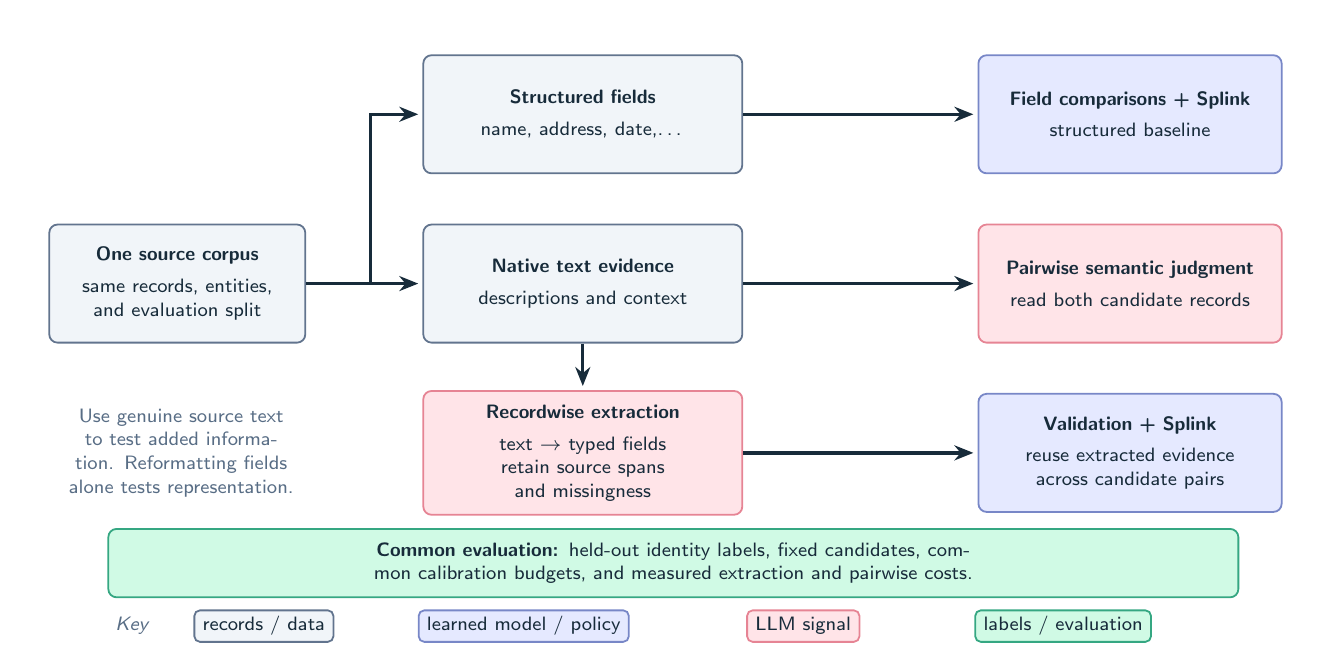
\begin{tikzpicture}

\useasboundingbox (-.2,.3) rectangle (16.1,-7.5);
\node[data,text width=29mm,minimum height=15mm] (records) at (1.7,-2.95) {\textbf{One source corpus}\\[3pt]same records, entities,\\and evaluation split};
\node[data,text width=37mm,minimum height=15mm] (fields) at (6.85,-.8) {\textbf{Structured fields}\\[3pt]name, address, date,\ldots};
\node[model,text width=35mm,minimum height=15mm] (fs) at (13.8,-.8) {\textbf{Field comparisons + Splink}\\[3pt]structured baseline};
\node[data,text width=37mm,minimum height=15mm] (text) at (6.85,-2.95) {\textbf{Native text evidence}\\[3pt]descriptions and context};
\node[llm,text width=35mm,minimum height=15mm] (direct) at (13.8,-2.95) {\textbf{Pairwise semantic judgment}\\[3pt]read both candidate records};
\node[llm,text width=37mm,minimum height=15mm] (extract) at (6.85,-5.1) {\textbf{Recordwise extraction}\\[3pt]text $\rightarrow$ typed fields\\retain source spans and missingness};
\node[model,text width=35mm,minimum height=15mm] (efs) at (13.8,-5.1) {\textbf{Validation + Splink}\\[3pt]reuse extracted evidence\\across candidate pairs};
\draw[route] (records.east) -- (4.15,-2.95);
\draw[flow] (4.15,-2.95) |- (fields.west); \draw[flow] (4.15,-2.95) -- (text.west);
\draw[flow] (fields) -- (fs); \draw[flow] (text) -- (direct); \draw[flow] (extract) -- (efs);
\draw[flow] (text.south) -- (extract.north);
\node[word,text width=33mm] at (1.75,-5.1) {Use genuine source text to test added information. Reformatting fields alone tests representation.};
\node[truth,text width=140mm] at (8,-6.5) {\textbf{Common evaluation:} held-out identity labels, fixed candidates, common calibration budgets, and measured extraction and pairwise costs.};
\rolekey{8}{-7.3}

\end{tikzpicture}
\end{document}
